\subsection{Fixpoint definition for approximations}

When using the definitions
  \ref{def:identity_lower_approximation} and
  \ref{def:identity_higher_approximation}
  for determining the rought set represention,
  we do not always get the most optimal solution.
We will illustrate this with the example depicted
  in figure \ref{fig:fixpoint}.

\begin{figure}
\label{fig:fixpoint}
\centering
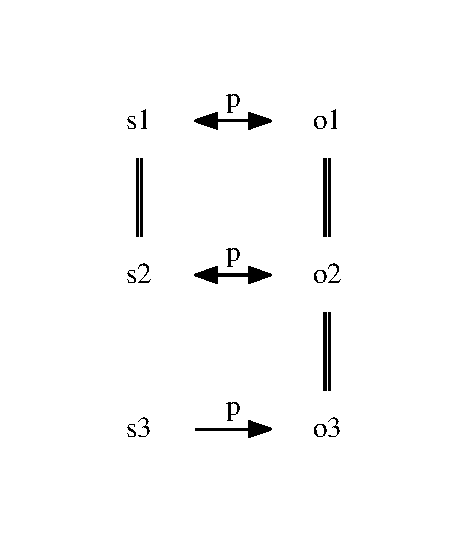
\includegraphics{./img/fixpoint_example}%[width=\columnwidth]
\caption{
  An illustrative example in which we show that defining
  $\lowerapprox$ in terms of $\higherapprox$ may not be optimal.
  The identity relation is represented with double-lined edges.
}
\end{figure}

The indiscernibility criteria for this example are shown
  in equation \ref{eq:20}.

\begin{align}
\label{eq:20}
  \indp_{\approx}(\set{s_1,s_2,s_3})
&=\\
  \indp_{\approx}(\set{o_1,o_2})
&=
  \setdef{p^n}{\natnum{n}}\nonumber
\end{align}

Based on these indiscernibility criteria the naive lower approximation
  (definition \ref{def:identity_lower_approximation}) is empty.
But notice that there is a slight asymmetry in the way in which we have
  calculated this result.
We have defined $\lowerapprox$ in terms of $\indp_{\approx}$,
  i.e. in terms of $\approx$.
It seems more correct, however, to base the indiscernibility criteria
  for calculating the lower approximation on $\lowerapprox$ itself
  (and similarly for the higher approximation).
The resulting definition \ref{def:identity_lower_approximation_fixpoint}
  is circular.
It affects the closure operations over the predicate and object terms
  in definition \ref{def:indiscernibility_predicates}.

\begin{definition}
\label{def:identity_lower_approximation_fixpoint}
\begin{align}
  x \in \lowerapprox
\, \iff \,
    \setdef{y}{x \equiv_{\indp_{\lowerapprox}} y}
  \; \subseteq \;
    \approx\nonumber
\end{align}
\end{definition}

There are now two correct solutions or fixpoints for the present example:

The first solution is the same as for the naive definition;
  $\lowerapprox_1 = \emptyset$,
  where $\indp_{\lowerapprox_1}(X) = \emptyset$
  for $X$ such that $\card{X} > 1$.

The second solution could not be derived in the naive case:
  $\lowerapprox_2 = \set{\pair{s_1}{s_2},\pair{o_1}{o_2}}$,
  with $\indp_{\lowerapprox_2}(\set{s_1,s_2,o_1,o_2}) = \setdef{p^n}{\natnum{n}}$
  and $\indp_{\lowerapprox_1}(X) = \emptyset$
  for all other $X$ such that $\card{X} > 1$.
This is the greatest fixpoint for this example.

Both solutions are correct,
  since both conform to the same strictures imposed by the here presented
  framework.
However, the second solution is better, since a greater fixpoint is
  to be prefered over a smaller fixpoint.
This both intuitively the case
  (since this enlarges the number of consistently applied identity pairs),
  and can be glanced from the quality criterion defined in \ref{def:quality}.
Reasoning along the same line,
  a least fixpoint\footnote{
    We have no reason to believe that it should be unique.
  } is the best solution for the redefined higher approximation.
